\documentclass{beamer}
\usepackage[utf8]{inputenc}
\usepackage{graphicx, epsfig}
\usepackage{amsmath,mathrsfs,amsfonts,amssymb}
\usepackage{floatflt}
\usepackage{epic,ecltree}
\usepackage{mathtext}
\usepackage{fancybox}
\usepackage{fancyhdr}
\usepackage{multirow}
\usepackage{enumerate}
\usepackage{epstopdf}
\usepackage{multicol}
\usepackage{algorithm}
\usepackage[noend]{algorithmic}
\usepackage{tikz}
\usepackage{blindtext}
\usetheme{default}%{Singapore}%{Warsaw}%{Warsaw}%{Darmstadt}
\usecolortheme{default}

\setbeamerfont{title}{size=\Huge}
\setbeamertemplate{footline}[page number]{}

\setbeamertemplate{section in toc}[sections numbered]


\makeatletter
\newcommand\HUGE{\@setfontsize\Huge{35}{40}}
\makeatother    

\setbeamerfont{title}{size=\HUGE}
\beamertemplatenavigationsymbolsempty

% latin bold lower
\newcommand{\ba}{\mathbf{a}} 
\newcommand{\bc}{\mathbf{c}} 
\newcommand{\be}{\mathbf{e}} 
\newcommand{\bff}{\mathbf{f}} % \bf - for bold type
\newcommand{\bg}{\mathbf{g}} 
\newcommand{\bh}{\mathbf{h}} 
\newcommand{\bp}{\mathbf{p}} 
\newcommand{\bq}{\mathbf{q}} 
\newcommand{\bt}{\mathbf{t}} 
\newcommand{\bs}{\mathbf{s}} 
\newcommand{\bu}{\mathbf{u}} 
\newcommand{\bv}{\mathbf{v}} 
\newcommand{\bw}{\mathbf{w}} 
\newcommand{\bx}{\mathbf{x}} 
\newcommand{\by}{\mathbf{y}} 
\newcommand{\bz}{\mathbf{z}} 

% latin bold upper
\newcommand{\bA}{\mathbf{A}} 
\newcommand{\bB}{\mathbf{B}} 
\newcommand{\bC}{\mathbf{C}} 
\newcommand{\bG}{\mathbf{G}} 
\newcommand{\bI}{\mathbf{I}} 
\newcommand{\bJ}{\mathbf{J}} 
\newcommand{\bL}{\mathbf{L}} 
\newcommand{\bM}{\mathbf{M}} 
\newcommand{\bP}{\mathbf{P}}
\newcommand{\bQ}{\mathbf{Q}} 
\newcommand{\bR}{\mathbf{R}} 
\newcommand{\bT}{\mathbf{T}} 
\newcommand{\bU}{\mathbf{U}} 
\newcommand{\bV}{\mathbf{V}} 
\newcommand{\bW}{\mathbf{W}} 
\newcommand{\bX}{\mathbf{X}} 
\newcommand{\bY}{\mathbf{Y}} 
\newcommand{\bZ}{\mathbf{Z}} 

% latin cal upper
\newcommand{\cF}{\mathcal{F}} 
\newcommand{\cG}{\mathcal{G}} 
\newcommand{\cI}{\mathcal{I}} 
\newcommand{\cL}{\mathcal{L}} 
\newcommand{\cM}{\mathcal{M}} 
\newcommand{\cN}{\mathcal{N}} 
\newcommand{\cP}{\mathcal{P}} 
\newcommand{\cS}{\mathcal{S}} 
\newcommand{\cT}{\mathcal{T}} 
\newcommand{\cW}{\mathcal{W}} 
\newcommand{\cX}{\mathcal{X}} 
\newcommand{\cZ}{\mathcal{Z}} 

% latin bb upper
\newcommand{\bbE}{\mathbb{E}} 
\newcommand{\bbI}{\mathbb{I}} 
\newcommand{\bbP}{\mathbb{P}} 
\newcommand{\bbR}{\mathbb{R}} 

% greek bold lower
\newcommand{\bepsilon}{\boldsymbol{\epsilon}} 
\newcommand{\btheta}{\boldsymbol{\theta}} 
\newcommand{\blambda}{\boldsymbol{\lambda}} 
\newcommand{\bpi}{\boldsymbol{\pi}} 
\newcommand{\bmu}{\boldsymbol{\mu}} 
\newcommand{\bsigma}{\boldsymbol{\sigma}} 
\newcommand{\bphi}{\boldsymbol{\phi}} 

% greek bold upper
\newcommand{\bSigma}{\boldsymbol{\Sigma}} 

\DeclareMathOperator*{\argmin}{arg\,min}
\DeclareMathOperator*{\argmax}{arg\,max}

\newcommand{\createdgmtitle}[1]{\title[\hbox to 56mm{Deep Generative Models  \hfill\insertframenumber\,/\,\inserttotalframenumber}]
	{\vspace{1cm} \\ \textbf{Deep Generative Models} \\ {\Huge Lecture #1}}
	\author{Roman Isachenko}
		\institute{
\includegraphics[width=0.7cm]{../utils/aimasterslogo} \LARGE{AI Masters}}
	\date{2024, Spring}
}

\usepackage{tikz}
\usetikzlibrary{arrows,shapes,positioning,shadows,trees}

\newcommand\myfootnote[1]{%
  \tikz[remember picture,overlay]
  \draw (current page.south west) +(1in + \oddsidemargin,0.5em)
  node[anchor=south west,inner sep=0pt]{\parbox{\textwidth}{%
      \rlap{\rule{10em}{0.4pt}}\raggedright\scriptsize \textit{#1}}};}

\newcommand\myfootnotewithlink[2]{%
  \tikz[remember picture,overlay]
  \draw (current page.south west) +(1in + \oddsidemargin,0.5em)
  node[anchor=south west,inner sep=0pt]{\parbox{\textwidth}{%
      \rlap{\rule{10em}{0.4pt}}\raggedright\scriptsize\href{#1}{\textit{#2}}}};}
      
\AtBeginSection[]
      {
      	\begin{frame}{Outline}
      		\tableofcontents[currentsection]
      	\end{frame}
      }
      \AtBeginSubsection[]{
      	\begin{frame}{Outline}
      		\tableofcontents[currentsection,currentsubsection]
      	\end{frame}
}
\createdgmtitle{13}

\usepackage{tikz}

\usetikzlibrary{arrows,shapes,positioning,shadows,trees}
%--------------------------------------------------------------------------------
\begin{document}
%--------------------------------------------------------------------------------
\begin{frame}[noframenumbering,plain]
%\thispagestyle{empty}
\titlepage
\end{frame}
%=======
\begin{frame}{Outline}
	\tableofcontents
\end{frame}
%=======
\begin{frame}{Recap of previous lecture}
	\vspace{-0.5cm}
	\[
		d\bx = \mathbf{f}(\bx, t) dt + g(t) d \bw - \text{SDE with the probability path } p_t(\bx)
	\]
	\vspace{-0.5cm}
	\begin{block}{Probability flow ODE}
		There exists ODE with identical the probability path $p_t(\bx)$ of the form
		\vspace{-0.3cm}
		\[
			d\bx = \left[\mathbf{f}(\bx, t) -\frac{1}{2} g^2(t) \frac{\partial}{\partial \bx} \log p_t(\bx) \right] dt
		\]
		\vspace{-0.3cm}
	\end{block}
	\begin{figure}
		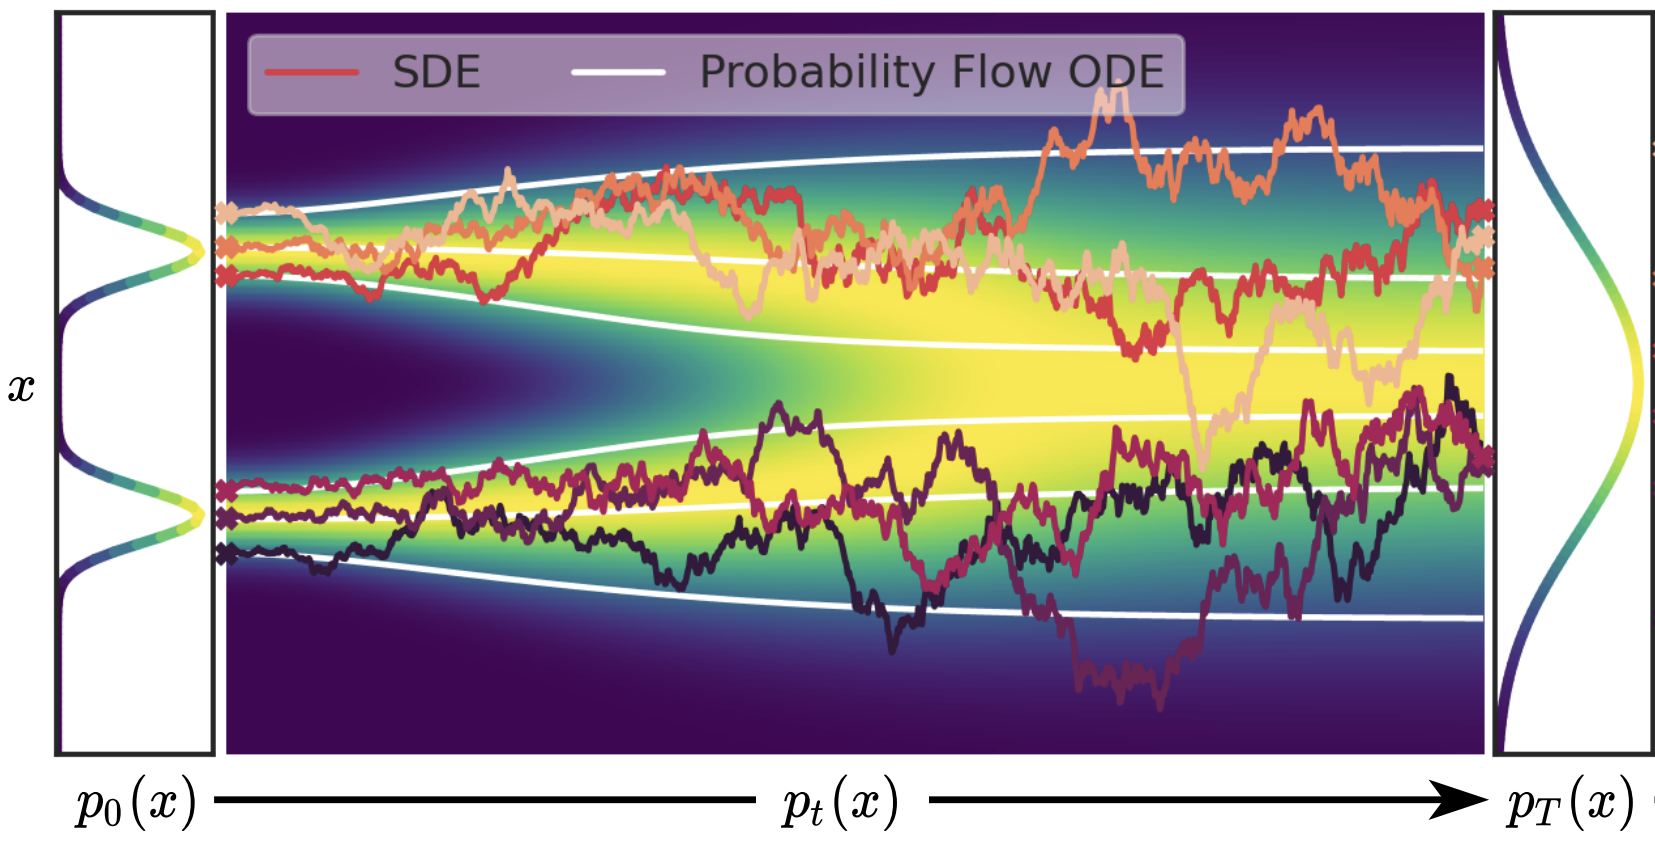
\includegraphics[width=0.75\linewidth]{figs/probability_flow}
	\end{figure}
	\myfootnotewithlink{https://arxiv.org/abs/2011.13456}{Song Y., et al. Score-Based Generative Modeling through Stochastic Differential Equations, 2020}
\end{frame}
%=======
\begin{frame}{Recap of previous lecture}
	\vspace{-0.3cm}
	\[
		d\bx = \mathbf{f}(\bx, t) dt, \quad \bx(t + dt) = \bx(t) + \mathbf{f}(\bx, t) dt
	\]
	\vspace{-0.5cm}
	\begin{block}{Reverse ODE}
		Let $\tau = 1 - t$ ($d\tau = -dt$).
		\vspace{-0.3cm}
		\[
			d\bx = - \bff(\bx, 1 - \tau) d \tau
		\]
	\end{block}
	\vspace{-0.5cm}
	\begin{block}{Reverse SDE}
		There exists the reverse SDE for the SDE $d\bx = \mathbf{f}(\bx, t) dt + g(t) d \bw$ that has the following form
		\vspace{-0.3cm}
		\[
			d\bx = \left(\mathbf{f}(\bx, t) {\color{violet}- g^2(t) \frac{\partial \log p_t(\bx)}{\partial \bx}}\right) dt + g(t) d \bw, \quad dt < 0
		\] 
	\end{block}
	\vspace{-0.5cm}
	\begin{block}{Sketch of the proof}
		\begin{itemize}
			\item Convert initial SDE to probability flow ODE.
			\item Revert probability flow ODE.
			\item Convert reverse probability flow ODE to reverse SDE.
		\end{itemize}
	\end{block}
	\myfootnotewithlink{https://arxiv.org/abs/2011.13456}{Song Y., et al. Score-Based Generative Modeling through Stochastic Differential Equations, 2020}
\end{frame}
%=======
\begin{frame}{Recap of previous lecture}
	\vspace{-0.5cm}
	\begin{align*}
		d\bx &= \mathbf{f}(\bx, t) dt + g(t) d \bw - \text{SDE} \\
		d\bx &= \left[\mathbf{f}(\bx, t) -\frac{1}{2} g^2(t) \frac{\partial}{\partial \bx} \log p_t(\bx) \right] dt - \text{probability flow ODE} \\
		d\bx &= \left(\mathbf{f}(\bx, t) - g^2(t) \frac{\partial \log p_t(\bx)}{\partial \bx}\right) dt + g(t) d \bw - \text{reverse SDE}
	\end{align*}
	\vspace{-0.5cm}
	\begin{itemize}
		\item We got the way to transform one distribution to another via SDE with some probability path $p_t(\bx)$.
		\item We are able to revert this process with the score function.
	\end{itemize}
	\vspace{-0.3cm}
	\begin{figure}
		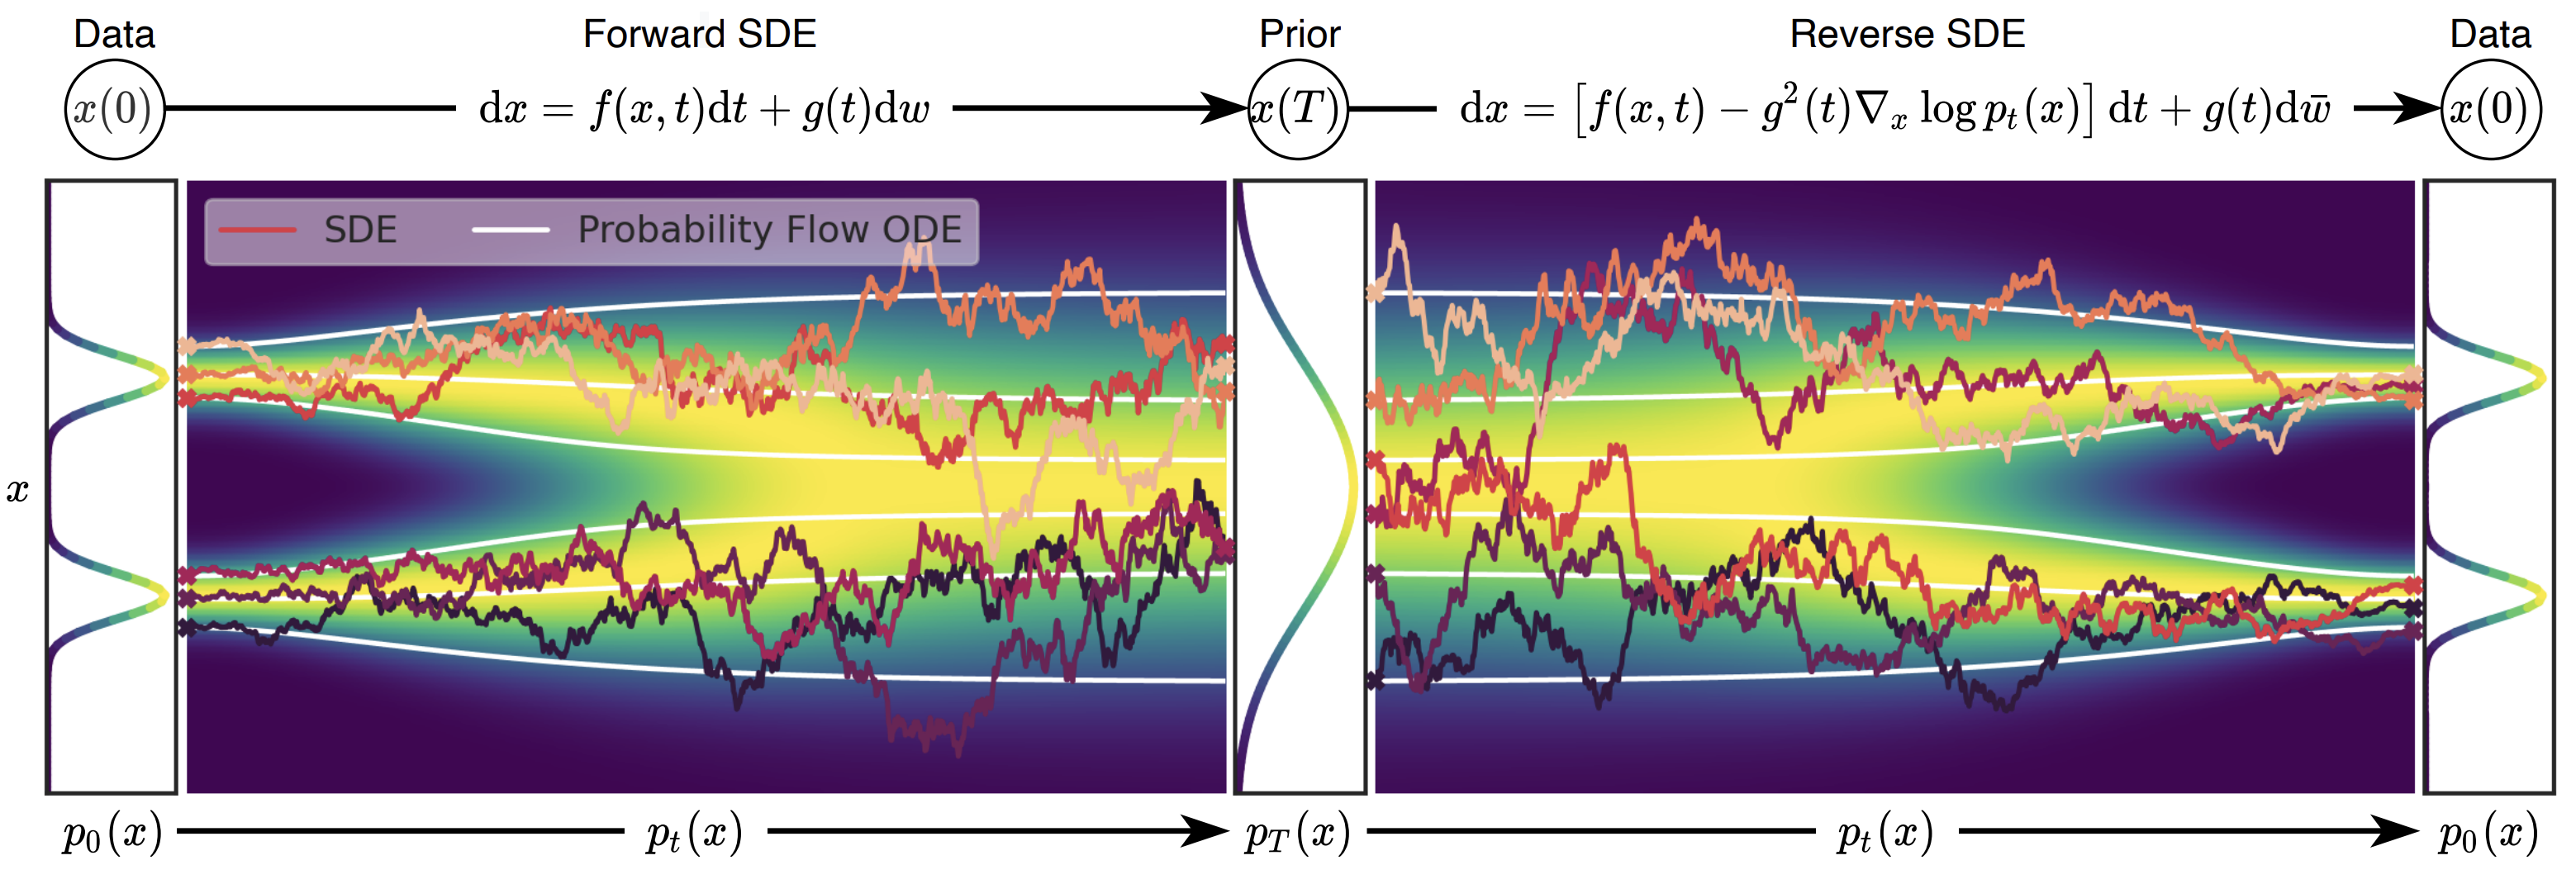
\includegraphics[width=0.9\linewidth]{figs/sde}
	\end{figure}
	\myfootnotewithlink{https://arxiv.org/abs/2011.13456}{Song Y., et al. Score-Based Generative Modeling through Stochastic Differential Equations, 2020}
\end{frame}
%=======
\begin{frame}{Recap of previous lecture}
	\vspace{-0.3cm}
	\[
		d\bx = \mathbf{f}(\bx, t) dt + g(t) d \bw
	\]
	\vspace{-0.3cm}
	\begin{block}{Variance Exploding SDE (NCSN)}
		\vspace{-0.5cm}
		\[
			d \bx = \sqrt{\frac{ d [\sigma^2(t)]}{dt}} \cdot d \bw, \quad \bff(\bx, t) = 0, \quad g(t) = \sqrt{\frac{ d [\sigma^2(t)]}{dt}} 
		\]
		Variance grows since $\sigma(t)$ is a monotonically increasing function.
	\end{block}
	\begin{block}{Variance Preserving SDE (DDPM)}
		\vspace{-0.3cm}
		\[
			d \bx = - \frac{1}{2} \beta(t) \bx(t) dt + \sqrt{\beta(t)} \cdot d \bw
		\]
		\[
			\bff(\bx, t) = - \frac{1}{2} \beta(t) \bx(t) , \quad g(t) = \sqrt{\beta(t)} 
		\]
		Variance is preserved if $\bx(0)$ has a unit variance.
	\end{block}
	\myfootnotewithlink{https://arxiv.org/abs/2011.13456}{Song Y., et al. Score-Based Generative Modeling through Stochastic Differential Equations, 2020}
\end{frame}
%=======
\section{Flow Matching}
%=======
\begin{frame}{Flow Matching}
	Let consider ODE dynamic $\bx_t = \bx(t)$ in time interval $t \in [0, 1]$ with boundaries $\bx_0 \sim p_0(\bx) = p(\bx)$, $\bx_1 \sim p_1(\bx) =  \pi(\bx)$. Here $p(\bx)$ is a base distribution ($\cN(0, \bI)$) and $\pi(\bx)$ is a true data distribution.
	\[
		\frac{d \bx}{dt} = \bu (\bx, t),
	\]
	$\bu (\bx, t): \bbR^m \times [0, 1] \rightarrow \bbR^m$ is a vector field.
	\[
		\frac{\partial p_t(\bx)}{\partial t} = - \text{div}\left(\bu(\bx, t) p_t(\bx)\right) 
	\]
	
	If we know the true vector field $\bu (\bx, t)$, then KFP equation gives us the way to compute the density $p_t(\bx)$.
	\begin{block}{Flow Matching}
		\[
			\bbE_{t \sim U[0, 1]} \bbE_{\bx \sim p_t(\bx)}\left\| \bu(\bx, t) - \bu_{\btheta}(\bx, t) \right\|^2 \rightarrow \min_{\btheta}
		\]
	\end{block}
	\myfootnotewithlink{https://arxiv.org/abs/2210.02747}{Lipman Y., et al. Flow Matching for Generative Modeling, 2022}
\end{frame}
%=======
\begin{frame}{Flow Matching}
	There exists infinite number of possible $\bu(\bx, t)$ between $\pi(\bx)$ and $p(\bx)$.
	\begin{minipage}[t]{0.45\columnwidth}
		\begin{figure}
			\centering
			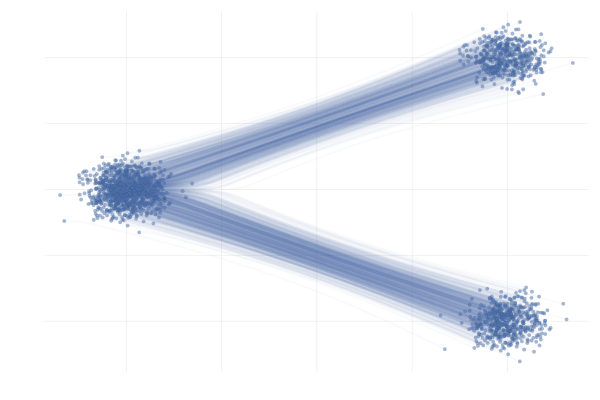
\includegraphics[width=\linewidth]{figs/non_uniqueness1}
		\end{figure}
	\end{minipage}%
	\begin{minipage}[t]{0.53\columnwidth}
		\begin{figure}
			\centering
			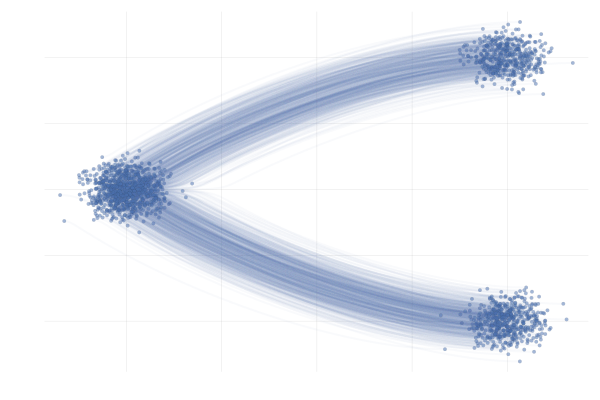
\includegraphics[width=\linewidth]{figs/non_uniqueness2}
		\end{figure}
	\end{minipage}
	\myfootnotewithlink{https://mlg.eng.cam.ac.uk/blog/2024/01/20/flow-matching.html}{image credit: https://mlg.eng.cam.ac.uk/blog/2024/01/20/flow-matching.html}
\end{frame}
%=======
\begin{frame}{Flow Matching}
	\[
		p_t(\bx) = \int p_t(\bx | \bz) p(\bz) d \bz 
	\]
	Here $p_t(\bx | \bz)$ is a \textbf{conditional probability path}.
	
	The conditional probability path $p_t(\bx | \bz)$ satisfies KFP theorem
	\[
		{\color{violet}\frac{\partial p_t(\bx | \bz)}{\partial t} = - \text{div}\left(\bu(\bx, \bz, t) p_t(\bx | \bz)\right)},
	\]
	where $\bu(\bx, \bz, t)$ is a \textbf{conditional vector field}.
	\[
		\frac{d\bx}{dt} = \bu(\bx, t) \quad \Rightarrow \quad \frac{d\bx}{dt} = \bu(\bx, \bz, t)
	\]
	\vspace{-0.3cm}
	\myfootnotewithlink{https://arxiv.org/abs/2302.00482}{Tong A., et al. Improving and Generalizing Flow-Based Generative Models with Minibatch Optimal Transport, 2023}
\end{frame}
%=======
\begin{frame}{Flow Matching}
	\[
		{\color{violet}\frac{\partial p_t(\bx | \bz)}{\partial t} = - \text{div}\left(\bu(\bx, \bz, t) p_t(\bx | \bz)\right)},
	\]
	\begin{block}{Theorem}
		\vspace{-0.3cm}
		\[
			\bu(\bx, t) = {\color{teal}\int \bu(\bx, \bz, t)} \frac{\color{teal}p_t(\bx | \bz) p(\bz)}{p_t(\bx)} {\color{teal}d \bz}
		\]
		\vspace{-0.4cm}
	\end{block}
	\begin{block}{Proof}
		\vspace{-0.5cm}
		\begin{multline*}
			\frac{\partial p_t(\bx)}{\partial t} = \frac{\partial}{\partial t} \int p_t(\bx | \bz) p(\bz) d \bz =  \int \left( {\color{violet} \frac{\partial p_t(\bx | \bz)}{\partial t} } \right) p(\bz) d \bz = \\
			= \int \left( {\color{violet} - \text{div}\left(\bu(\bx, \bz, t) p_t(\bx | \bz)\right) } \right) p(\bz) d \bz = \\
			= - \text{div} \left({\color{teal}\int \bu(\bx, \bz, t) p_t(\bx | \bz) p(\bz) d \bz }\right) = - \text{div}  \left(\bu(\bx, t) p_t(\bx)\right)
		\end{multline*}
	\end{block}
	\myfootnotewithlink{https://arxiv.org/abs/2302.00482}{Tong A., et al. Improving and Generalizing Flow-Based Generative Models with Minibatch Optimal Transport, 2023}
\end{frame}
%=======
\begin{frame}{Flow Matching}
	\begin{block}{Flow Matching}
		\[
			\bbE_{t \sim U[0, 1]} \bbE_{\bx \sim p_t(\bx)}\left\| \bu(\bx, t) - \bu_{\btheta}(\bx, t) \right\|^2 \rightarrow \min_{\btheta}
		\]
	\end{block}
	\begin{block}{Conditional Flow Matching}
		\[
			\bbE_{t \sim U[0, 1]} \bbE_{\bz \sim p(\bz)} \bbE_{\bx \sim p_t(\bx | \bz)}\left\| \bu(\bx, \bz, t) - \bu_{\btheta}(\bx, t) \right\|^2 \rightarrow \min_{\btheta}
		\]
	\end{block}
	\begin{block}{Theorem}
		If $\text{supp}(p_t(\bx)) = \bbR^m$, then the optimal value of FM objective is equal to the optimal value of CFM objective.
	\end{block}
	\begin{block}{Proof}
		It is proved similarly with the denoising score matching theorem.
	\end{block}
	\myfootnotewithlink{https://arxiv.org/abs/2302.00482}{Tong A., et al. Improving and Generalizing Flow-Based Generative Models with Minibatch Optimal Transport, 2023}
\end{frame}
%=======
\begin{frame}{Flow Matching}
	\begin{block}{Gaussian conditional probability path}
		\vspace{-0.3cm}
		\[
			p_t(\bx | \bz) = \cN\left(\bmu_t(\bz), \bsigma_t^2(\bz)\right)
		\]
		\vspace{-0.6cm}
	\end{block}
	\myfootnotewithlink{https://arxiv.org/abs/2302.00482}{Tong A., et al. Improving and Generalizing Flow-Based Generative Models with Minibatch Optimal Transport, 2023}
\end{frame}
%=======

\subsection{Endpoint conditioning}
%=======
\begin{frame}{Flow Matching}
	\begin{block}{Conditional Flow Matching}
		\vspace{-0.3cm}
		\[
			\bbE_{t \sim U[0, 1]} \bbE_{\bz \sim p(\bz)} \bbE_{\bx \sim p_t(\bx | \bz)}\left\| \bu(\bx, \bz, t) - \bu_{\btheta}(\bx, t) \right\|^2 \rightarrow \min_{\btheta}
		\]
	\end{block}
	Let choose $\bz = \bx_1$. Then $p(\bz) = p_1(\bx_1)$.
	\[
		p_t(\bx) = \int p_t(\bx | \bx_1) p_1(\bx_1) d \bx_1
	\]
	We need to ensure boundary conditions:
	\[
		p_0(\bx | \bx_1) = p_0(\bx); \quad p_1(\bx | \bx_1) = \delta(\bx - \bx_1)
	\]
	\vspace{-0.3cm}
	\begin{block}{Gaussian conditional probability path}
		\[
			p_t(\bx | \bx_1) = \cN\left(\bmu_t(\bx_1), \bsigma_t^2(\bx_1)\right)
		\]
		\vspace{-0.6cm}
	\end{block}
	\[
		\bmu_0(\bx_1) = 0, \quad \bsigma_0(\bx_1) = 1, \quad \bmu_1(\bx_1) = \bx_1, \quad \bsigma_1(\bx_1) = 0
	\]
	\myfootnotewithlink{https://arxiv.org/abs/2210.02747}{Lipman Y., et al. Flow Matching for Generative Modeling, 2022}
\end{frame}
%=======
\begin{frame}{Flow Matching}
	\begin{block}{Theorem}
		\[
			\bu(\bx, \bx_1, t) =  \bmu_t'(\bx_1) + \frac{\bsigma_t'(\bx_1)}{\bsigma_t(\bx_1)} \odot (\bx - \bmu_t(\bx_1))
		\]
	\end{block}
	\begin{block}{Proof}
	\[
		p_t(\bx | \bx_1) = \cN\left(\bmu_t(\bx_1), \bsigma_t^2(\bx_1)\right)
	\]
	\[
		\bx = \bmu_t(\bx_1) + \bsigma_t(\bx_1) \odot \bepsilon, \quad \Rightarrow \quad \bepsilon = \frac{1}{\bsigma_t(\bx_1)} \odot (\bx - \bmu_t(\bx_1))
	\]
	\[
		 \frac{d\bx}{dt} = \bu(\bx, \bx_1, t)
	\]
	\[
		\frac{d\bx}{dt} = \bmu_t'(\bx_1) + \bsigma_t'(\bx_1) \odot \bepsilon =  \bmu_t'(\bx_1) + \frac{\bsigma_t'(\bx_1)}{\bsigma_t(\bx_1)} \odot (\bx - \bmu_t(\bx_1))
	\]
	\end{block}
	\myfootnotewithlink{https://arxiv.org/abs/2210.02747}{Lipman Y., et al. Flow Matching for Generative Modeling, 2022}
\end{frame}
%=======
\begin{frame}{Flow Matching}
	\[
		\bu(\bx, \bx_1, t) =  \bmu_t'(\bx_1) + \frac{\bsigma_t'(\bx_1)}{\bsigma_t(\bx_1)} \odot (\bx - \bmu_t(\bx_1))
	\]
	\[
		\bmu_0(\bx_1) = 0, \quad \bsigma_0(\bx_1) = 1, \quad \bmu_1(\bx_1) = \bx_1, \quad \bsigma_1(\bx_1) = 0
	\]
	\[
		\bmu_t(\bx_1) = t \bx_1; \quad \bsigma_t(\bx_1) = (1 - t); \quad \bu(\bx, \bx_1, t) = \frac{\bx_1  - \bx}{1-t}
	\]
	\myfootnotewithlink{https://arxiv.org/abs/2210.02747}{Lipman Y., et al. Flow Matching for Generative Modeling, 2022}
\end{frame}
%=======
\begin{frame}{Flow Matching}
	\begin{figure}
		\centering
		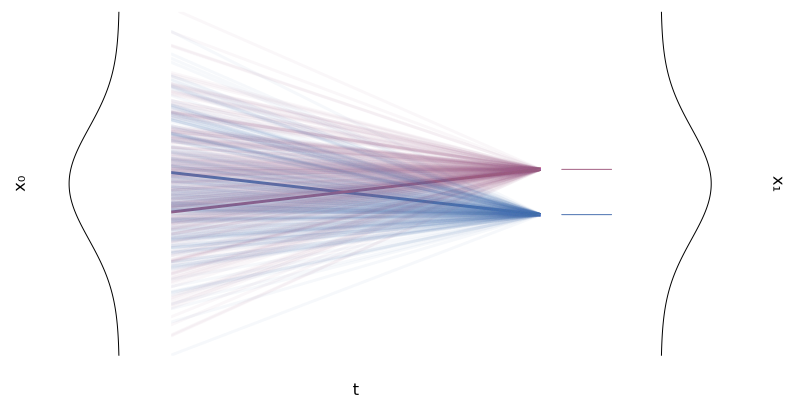
\includegraphics[width=\linewidth]{figs/heatmap_with_cond_traj-v3}
	\end{figure}
	\myfootnotewithlink{https://mlg.eng.cam.ac.uk/blog/2024/01/20/flow-matching.html}{image credit: https://mlg.eng.cam.ac.uk/blog/2024/01/20/flow-matching.html}
\end{frame}
%=======
\begin{frame}{Flow Matching}
	\begin{figure}
		\centering
		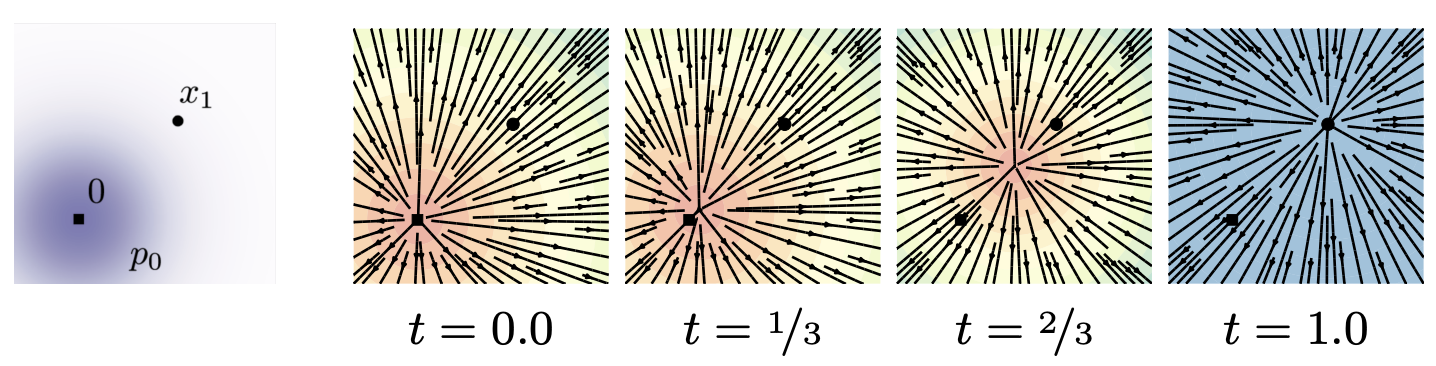
\includegraphics[width=\linewidth]{figs/diff_cond_path}
	\end{figure}
	\begin{figure}
		\centering
		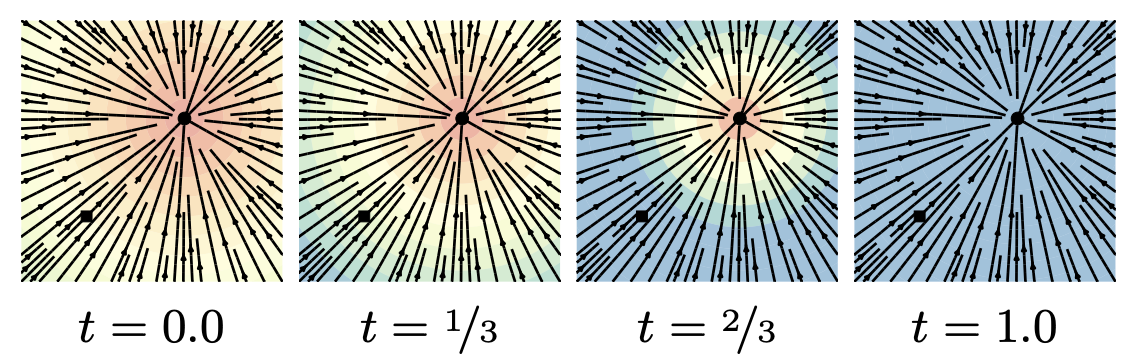
\includegraphics[width=\linewidth]{figs/ot_cond_path}
	\end{figure}
	\myfootnotewithlink{https://arxiv.org/abs/2210.02747}{Lipman Y., et al. Flow Matching for Generative Modeling, 2022}
\end{frame}
%=======
\begin{frame}{Flow Matching}
	\begin{figure}
		\centering
		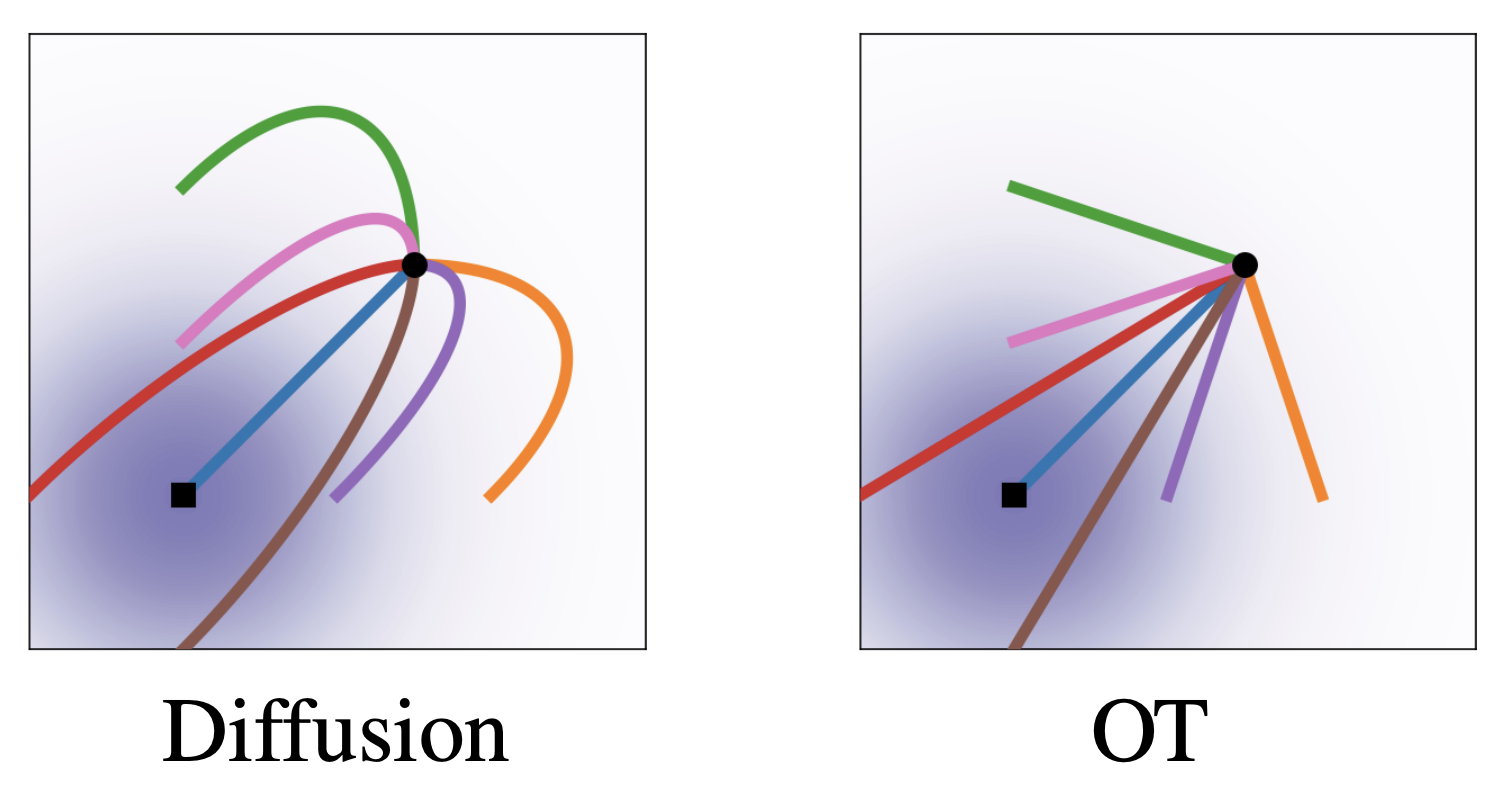
\includegraphics[width=\linewidth]{figs/trajectories}
	\end{figure}
	\myfootnotewithlink{https://arxiv.org/abs/2210.02747}{Lipman Y., et al. Flow Matching for Generative Modeling, 2022}
\end{frame}
%=======
\subsection{Pair conditioning}
%=======
\begin{frame}{Summary}
	\begin{itemize}
		\item
	\end{itemize}
\end{frame}
\end{document} 